\hypertarget{cif_cifPres}{}\section{Presentation}\label{cif_cifPres}
The {\bfseries Caltech Intermediate Format (C\-I\-F)} consists in a limited set of graphic primitives used to describe the shapes on each layer of an integrated circuit (see \href{http://en.wikipedia.org/wiki/Caltech_Intermediate_Form}{\tt http\-://en.\-wikipedia.\-org/wiki/\-Caltech\-\_\-\-Intermediate\-\_\-\-Form} for more informations). \par
 \hypertarget{cif_cifAutrhos}{}\subsection{Author}\label{cif_cifAutrhos}
Damien Dupuis\-: damien.\-dupuis(at)lip6(.)fr\hypertarget{cif_cifLimits}{}\subsection{Limitations}\label{cif_cifLimits}
Although the C\-I\-F format allows hierarchical description and supports several shapes, in this driver, we do not use hierarchy and only use Polygons.\hypertarget{cif_cifDB}{}\section{Stand alone database structure}\label{cif_cifDB}
The database consists in two simple objects \-:
\begin{DoxyItemize}
\item \hyperlink{class_c_i_f_1_1_circuit}{C\-I\-F\-::\-Circuit} contains all C\-I\-F circuit informations such as the name, the unit used, the scale and the list of all Polygons.
\item \hyperlink{class_c_i_f_1_1_polygon}{C\-I\-F\-::\-Polygon} describes a Polygon (a set of points).
\end{DoxyItemize}\hypertarget{cif_cifDriver}{}\subsection{Using the driver}\label{cif_cifDriver}
To drive a C\-I\-F file, user has to create one \hyperlink{class_c_i_f_1_1_circuit}{C\-I\-F\-::\-Circuit} and as many \hyperlink{class_c_i_f_1_1_polygon}{C\-I\-F\-::\-Polygon} as the number of shapes of the layout. The \hyperlink{class_c_i_f_1_1_polygon}{C\-I\-F\-::\-Polygon} objects can be created independently from for the \hyperlink{class_c_i_f_1_1_circuit}{C\-I\-F\-::\-Circuit} but must be finally added to the \hyperlink{class_c_i_f_1_1_circuit}{C\-I\-F\-::\-Circuit} using \hyperlink{class_c_i_f_1_1_circuit_a5b37e86206e2a128ba6db4987dc09a39}{C\-I\-F\-::\-Circuit\-::add\-Polygon()}.\par
Once the \hyperlink{class_c_i_f_1_1_circuit}{C\-I\-F\-::\-Circuit} is complete, simply call the \hyperlink{class_c_i_f_1_1_circuit_a90c823b70c4984f302c19ceca604d101}{C\-I\-F\-::\-Circuit\-::write\-To\-File()} method to drive the database to file.\hypertarget{cif_cifExamples}{}\section{Examples}\label{cif_cifExamples}
As said is the global presentation, V\-L\-S\-I S\-A\-P\-D project provides C++ libraries and Python modules for each supported format. In this section we present two simple code examples to drive a C\-I\-F file using C++ or Python. These two examples drive the same file {\ttfamily transistor.\-cif\-:} 
\begin{DoxyCodeInclude}
(CIF file written on 11-Jun-2010  13:49:44 by VLSISAPD\_CIF\_DRIVER);
(Units: micro  -  UU/DB Scale: 0.001);
DS 1 1 1;
9 Transistor;
L 6; P 130,290 540,290 540,690 130,690;
L 17; P 305,150 365,150 365,830 305,830;
DF;
C 1;
E
\end{DoxyCodeInclude}


 
\begin{DoxyImage}
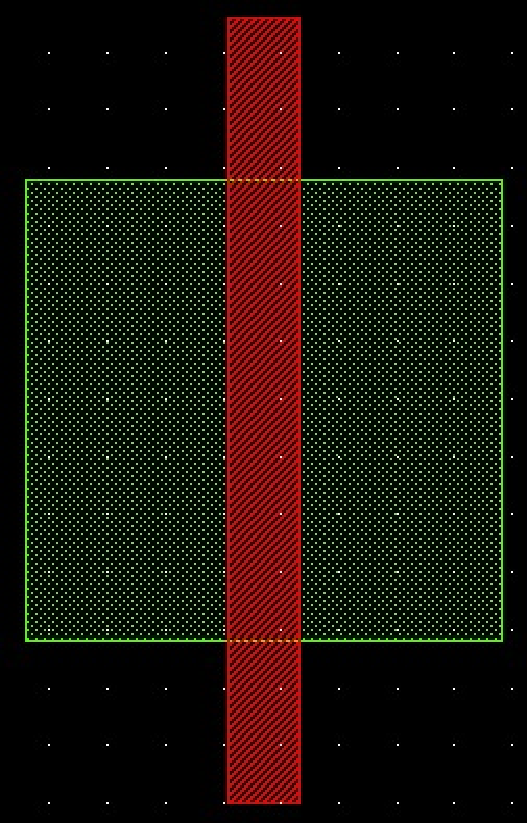
\includegraphics{transistorCif}
\caption{C\-I\-F example layout width=.25}
\end{DoxyImage}
\hypertarget{cif_cifC}{}\subsection{C++}\label{cif_cifC}
Here is the C++ code ({\ttfamily drive\-Cif.\-cpp}) used to generate the transistor.\-cif file. (Source is available in examples directory). 
\begin{DoxyCodeInclude}
\textcolor{preprocessor}{#include <string>}
\textcolor{keyword}{using namespace }std;

\textcolor{preprocessor}{#include "vlsisapd/cif/Circuit.h"}
\textcolor{preprocessor}{#include "vlsisapd/cif/Polygon.h"}

\textcolor{keywordtype}{int} main(\textcolor{keywordtype}{int} argc, \textcolor{keywordtype}{char} * argv[]) \{
    \hyperlink{class_c_i_f_1_1_circuit}{CIF::Circuit}* circuit = \textcolor{keyword}{new} \hyperlink{class_c_i_f_1_1_circuit}{CIF::Circuit}(\textcolor{keywordtype}{string}(\textcolor{stringliteral}{"Transistor"}), \textcolor{keywordtype}{string}(\textcolor{stringliteral}{"micro"}),
       0.001);

    \textcolor{comment}{// Layer #6 corresponds to active}
    \hyperlink{class_c_i_f_1_1_polygon}{CIF::Polygon}* poly = \textcolor{keyword}{new} \hyperlink{class_c_i_f_1_1_polygon}{CIF::Polygon}(6);
    poly->\hyperlink{class_c_i_f_1_1_polygon_ab3047469780327f18539907e1303ea15}{addPoint}(130, 290);
    poly->\hyperlink{class_c_i_f_1_1_polygon_ab3047469780327f18539907e1303ea15}{addPoint}(540, 290);
    poly->\hyperlink{class_c_i_f_1_1_polygon_ab3047469780327f18539907e1303ea15}{addPoint}(540, 690);
    poly->\hyperlink{class_c_i_f_1_1_polygon_ab3047469780327f18539907e1303ea15}{addPoint}(130, 690);
    circuit->\hyperlink{class_c_i_f_1_1_circuit_a5b37e86206e2a128ba6db4987dc09a39}{addPolygon}(poly);

    \textcolor{comment}{// Layer #17 corresponds to polysilicium}
    poly = \textcolor{keyword}{new} \hyperlink{class_c_i_f_1_1_polygon}{CIF::Polygon}(17);
    poly->\hyperlink{class_c_i_f_1_1_polygon_ab3047469780327f18539907e1303ea15}{addPoint}(305, 150);
    poly->\hyperlink{class_c_i_f_1_1_polygon_ab3047469780327f18539907e1303ea15}{addPoint}(365, 150);
    poly->\hyperlink{class_c_i_f_1_1_polygon_ab3047469780327f18539907e1303ea15}{addPoint}(365, 830);
    poly->\hyperlink{class_c_i_f_1_1_polygon_ab3047469780327f18539907e1303ea15}{addPoint}(305, 830);
    circuit->\hyperlink{class_c_i_f_1_1_circuit_a5b37e86206e2a128ba6db4987dc09a39}{addPolygon}(poly);

    circuit->\hyperlink{class_c_i_f_1_1_circuit_a90c823b70c4984f302c19ceca604d101}{writeToFile}(\textcolor{stringliteral}{"./transistor.cif"});
    
    \textcolor{keywordflow}{return} 0;
\}

\end{DoxyCodeInclude}


\begin{DoxyNote}{Note}
In order to compile this code, a C\-Make\-Lists.\-txt file is provided. User must set the \$\-V\-L\-S\-I\-S\-A\-P\-D\-\_\-\-T\-O\-P variable before running these commands in the directory containing the C\-Make\-Lists.\-txt file\-: 
\begin{DoxyCode}
%> mkdir build; cd build
%> cmake ..
%> make
\end{DoxyCode}

\end{DoxyNote}
\hypertarget{cif_cifPython}{}\subsection{Python}\label{cif_cifPython}
Here is the Python code ({\ttfamily drive\-Cif.\-py}) used to generate the transistor.\-cif file. (Source is available in examples directory). 
\begin{DoxyCodeInclude}
1 \textcolor{keyword}{import} CIF
2 circuit = \hyperlink{class_c_i_f_1_1_circuit}{CIF.Circuit}(\textcolor{stringliteral}{"Transistor"}, \textcolor{stringliteral}{"micro"}, 0.001)
3 poly1 = \hyperlink{class_c_i_f_1_1_polygon}{CIF.Polygon}(6)
4 poly1.addPoint(130, 290)
5 poly1.addPoint(540, 290)
6 poly1.addPoint(540, 690)
7 poly1.addPoint(130, 690)
8 circuit.addPolygon(poly1)
9     
10 poly2 = \hyperlink{class_c_i_f_1_1_polygon}{CIF.Polygon}(17)
11 poly2.addPoint(305, 150);
12 poly2.addPoint(365, 150);
13 poly2.addPoint(365, 830);
14 poly2.addPoint(305, 830);
15 circuit.addPolygon(poly2)
16 
17 circuit.writeToFile(\textcolor{stringliteral}{"./transistor.cif"})
\end{DoxyCodeInclude}


\begin{DoxyNote}{Note}
In order to run the {\ttfamily drive\-Cif.\-py} script, user must ensure that \$\-P\-Y\-T\-H\-O\-N\-P\-A\-T\-H variable points to the directory containing C\-I\-F.\-so module. 
\end{DoxyNote}
